\chapter{Anomaly Detection} \label{chap:anomaly}

\section*{}

This chapter introduces the concept of \textit{Anomaly Detection} and includes an overview over the different types of techniques.

\section{Definition}

The following concept of Anomaly Detection is proposed, based on the one provided by \textcite{Kandhari2009}:

\begin{definition}[Anomaly Detection]
	Anomaly Detection (also known as Outlier Detection and Outlier Analysis) corresponds to the problem of finding patterns in data that do not conform to expected behavior.
\end{definition}

The objective is to find instances $d_o$, within a dataset $\mathcal{D}$, that deviate so much from other instances that raises suspicions of being generated from a different mechanism \cite{hawkins1980identification}.

It is also important to distinguish this field from other similar ones \cite{Kandhari2009}:
\begin{itemize}
	\item \textit{Noise removal} and \textit{noise accommodation}: where the goal is to detect and remove unwanted \textit{anomalies} (which are designated by \textit{noise}) that may affect the process of data analysis.
	
	\item \textit{Novelty detection}: where the goal is to find anomalous patterns that were not observed before and mark them afterwards as being \textit{normal} in the future (e.g. detecting emerging topics in social media).
\end{itemize}

%It is also important to mention that the terms \textit{anomaly} and \textit{outlier} are frequently used throughout the literature as being synonyms \cite{Kandhari2009}. %, although the ``outlier'' appears to be used more when referring to unsupervised anomaly detection approaches (SEE SECTION X).

%The field of Anomaly Detection has some taxonomy associated

A taxonomy was proposed by \textcite{Kandhari2009} regarding the following aspects in this field: type of anomalies, learning mode and type of techniques (categorized according to their underlying idea and assumptions).

\section{Type of Anomalies} \label{sec:anomaly_type}

Anomalies can be classified based on their nature into one of the following categories:

\begin{itemize}
	\item \textit{Point Anomaly:} when an individual data instance of a dataset can be considered anomalous, by comparing it with the rest of the dataset. This is the focus of the majority of the research in this field.
	
	\item \textit{Contextual Anomaly} or \textit{Conditional Anomaly}: When a individual data instance of a dataset can be considered anomalous when it is present in a certain context. This assumes that the dataset has attributes that can define a context (e.g. time -- in time series or GPS coordinates -- in spatial data). Figure \ref{fig:context_anom} illustrates this type of anomaly with a time series dataset regarding the monthly temperature over a year: although $t_1$ and $t_2$ have both the same temperature value, $t_2$ is considered a contextual anomaly.
	
	\begin{figure}[!ht]
		\centering
		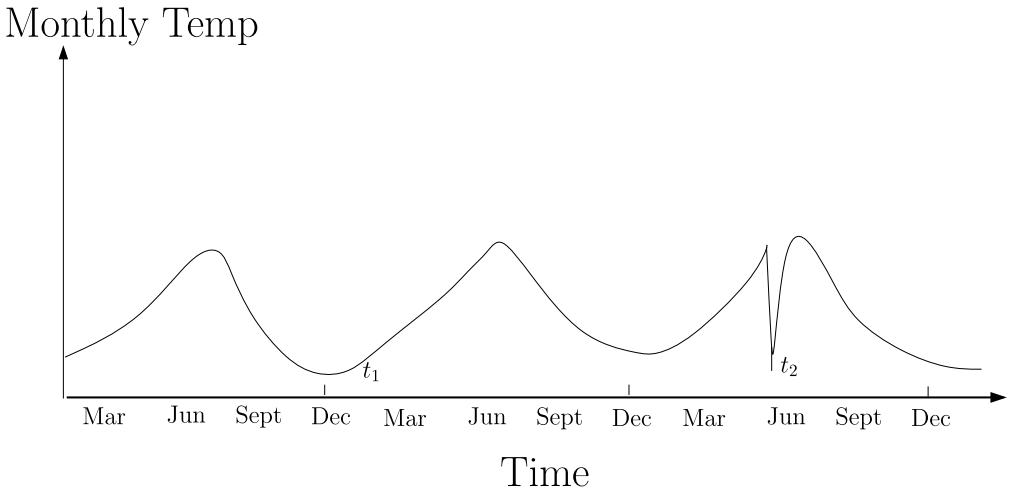
\includegraphics[width=0.7\textwidth]{contextual.png}
		\caption{Example of one contextual anomaly ($t_2$) in a monthly temperature time series dataset. Source: \cite{Kandhari2009}.}
		\label{fig:context_anom}
	\end{figure}
	
	\item \textit{Collective Anomaly}: When a group of data instances of a dataset may not be anomalies by themselves, but when they occur together they can be considered a collective anomaly.
	Figure \ref{fig:collective_anom} illustrates this type of anomaly using a human electrocardiogram output time series: the red values represent a collective anomaly, although that value by itself is not considered an anomaly (despite appearing several times during the dataset just by itself).
	
	\begin{figure}[!ht]
		\centering
		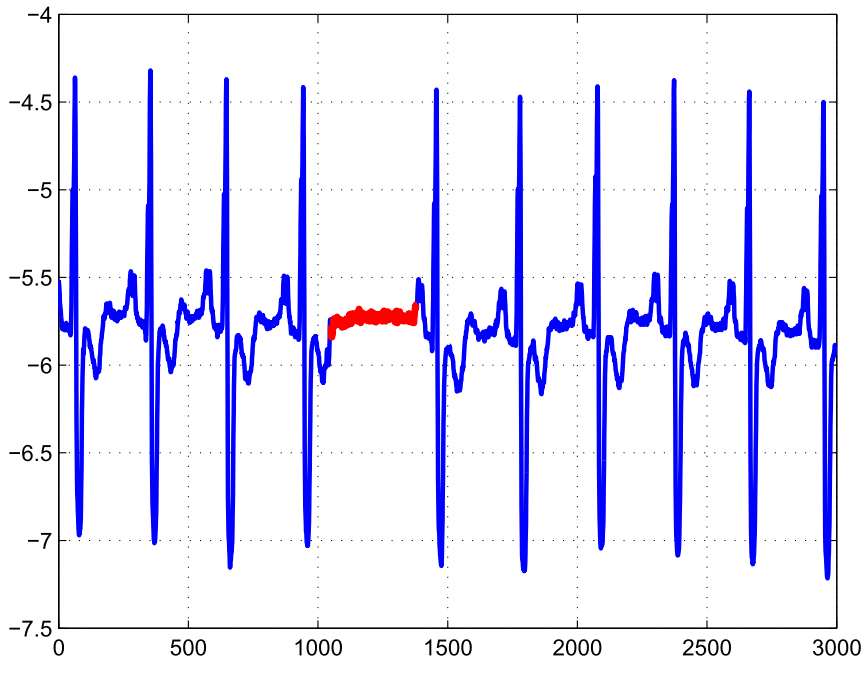
\includegraphics[width=0.6\textwidth]{collective.png}
		\caption{Example of one collective anomaly in a human electrocardiogram output time series dataset. Source:  \cite{Kandhari2009}.}
		\label{fig:collective_anom}
	\end{figure}
	
\end{itemize}

Because of the wide scope of each of these categories, this thesis will only focus on \textit{point anomalies} in the following sections and chapters. Information regarding the techniques capable of detecting contextual and collective anomalies can be found in Kandhari's survey on the topic (\cite{Kandhari2009}).

\section{Learning Mode} \label{sec:anomly_learn}

Anomaly Detection techniques can be classified based on the learning mode used:

\begin{itemize}
	\item \textit{Supervised}: Techniques using this learning mode assume that the data is fully labeled as either being \textit{normal} or \textit{anomalous}.
	Therefore, this constitutes a regular supervised learning classification problem. %However, it is important to note that in this case the classes are skewed (i.e. there will be have less anomalies in a dataset than \textit{normal} instances).
	
	\item \textit{Semi-supervised}: Techniques using this learning mode assume that the data only contains \textit{normal} examples and try to build a model that can learn the \textit{normal} behavior and identify examples that do not fit in this behavior.
	In the real-world this scenario is very frequent as in many domains it is difficult or expensive to measure anomalies and only \textit{normal} data is available.
	
	\item \textit{Unsupervised}: This learning mode does not require labeled data and assumes that the number of \textit{normal} instances is much higher than the number of \textit{anomalous} instances.
	Most of the Anomaly Detection techniques defined in the literature operate under this learning mode.
\end{itemize}


\section{Type of Techniques} \label{sec:anomaly_appr}

The techniques used in Anomaly Detection can be categorized into two groups according to their output \cite{Kandhari2009}:

\begin{itemize}
	\item \textit{Score output:} The techniques with this type of output assign a \textit{score} to each data instance that represents how much the instance can be considered an anomaly. The list of anomalous instances can then be retrieved by using manually defined thresholds on the scores or by marking all the top instances as \textit{anomalous}.
	
	\item \textit{Label output:} The techniques that output labels resemble regular binary-classifiers in Machine Learning by either classifying a data instance as being \textit{normal} or \textit{anomalous}. These techniques differentiate from the \textit{score} ones as they do not require any type of threshold definition after their application, as the data instance is already labeled as \textit{anomalous} or \textit{normal}.
\end{itemize}

\subsection{Classification Based Techniques}

Classification based techniques operate similarly to regular supervised learning classifiers: they train a model based on a set of labeled data and then classify each test data instance as being \textit{normal} or \textit{anomalous}.

One of the disadvantages of this group of techniques is that they require labeled data in the training phase of the model. Depending on the labels available in the training data, the techniques in this group can be subdivided into two types \cite{Kandhari2009}: multi-class and one-class.

%\textbf{TODO: Where does ``isolation forest'' algorithm fit?}

\subsubsection{Multi-class Techniques}\mbox{}

Multi-class techniques assume that the training data contains instances belonging to several different \textit{normal} classes and build a classifier that distinguishes each class from the remaining classes. These techniques classify a data instance as being \textit{anomalous} if they cannot classify it as one of the \textit{normal} classes \cite{Kandhari2009}.

Examples of these techniques include certain types of Neural Networks (e.g. Multi Layered Perceptrons, Hopfield Networks), Bayesian Networks, Rule Based techniques, Decision Trees and other binary and multi-class classifiers \cite{Kandhari2009}.

\subsubsection{One-class Techniques}\mbox{}

One-class techniques assume that the training data contains instances belonging to only one class -- the \textit{normal} one. The idea behind these techniques when learning the model is to define a decision boundary that isolates the \textit{normal} instances.
This decision boundary can therefore be used to classify new data: data instances that stay inside the decision boundry are are considered \textit{normal} and instances that stay outside the boundary are flagged as anomalies \cite{Kandhari2009}.
These techniques usually operate under the semi-supervised learning method presented in section \ref{sec:anomly_learn}.

Examples of these techniques include Replicator Neural Networks \cite{Hawkins}, Support Vector Machines (more specifically One-class SVMs \cite{Sc}) and Rule Based techniques \cite{Kandhari2009}).

\subsection{Nearest Neighbor Based Techniques}

Nearest Neighbor based techniques are based on the assumption that \textit{normal} data instances are situated in dense \textit{neighborhoods} of data instances, while \textit{anomalous} data instances situate themselves \textit{far} from other data instances.
The notion of \textit{neighboorhoods} and \textit{far} are employed with similarity/distance metrics that can evaluate how close (or far away) two data instances are.

These techniques can be subdivided into two different groups \cite{Kandhari2009}:
\begin{itemize}
	\item techniques that use the distance of each data instance to its $k^{th}$ nearest neighbor(s) as an anomaly score;
	
	\item techniques that use the concept of relative density of each data instance to compute an anomaly score (which will be detailed in this section).
\end{itemize}

\subsubsection{Density Techniques}\mbox{}

The assumption behind the density techniques is that a data instance that belongs to a neighborhood with low density (i.e. that contains only a few data instances) is \textit{anomalous}, while the opposite indicates that the instance is \textit{normal}.

\begin{figure}[!ht]
	\centering
	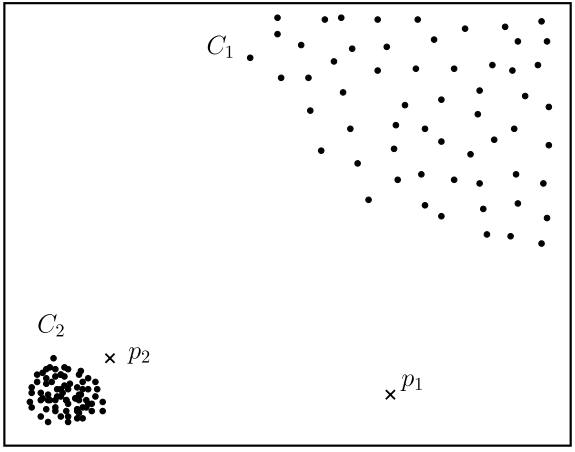
\includegraphics[width=0.6\textwidth]{density_anomalies.png}
	\caption{Example of a 2 dimensional dataset containing regions with different density values. Source: \cite{Kandhari2009}.}
	\label{fig:local_density}
\end{figure}

However, it is important to note that this assumption may not hold if the data has regions with different density values. Figure \ref{fig:local_density} illustrates this example with a 2 dimensional dataset: the distance of each of the instances in cluster $C_1$ to their nearest neighbor is higher than the distance of $p_2$ to its nearest neighbor in cluster $C_2$. Because of this the methods that are based on this assumption would not consider $p_2$ as an \textit{anomalous} instance although visually it is noticeable that this instance is \textit{anomalous} in the given feature space.

In order to overcome this limitation, some techniques within this category compare the density of the data instances to the density of their neighbors. One of the examples of this type of techniques is the LOF (Local Outlier Factor) \cite{Breunig}. Several techniques based on LOF	have been proposed more recently, either to adapt this algorithm to more complex data types or to improve its efficiency. Some examples include COF (Connectivity-based Outlier Factor) \cite{Tang2002}, ODIN (Outlier Detection using In-degree Number) \cite{Hautamaki2004} and LOCI (Local Correlation Integral) \cite{PapadimitriouS.KitagawaH.2003}.

\subsection{Clustering Based Techniques}

Clustering is a task in Data Mining in which the goal is to aggregate the data into meaningful or useful groups \cite{Tan2005}. Techniques that capture this idea have been applied to Anomaly Detection, out of which three groups of techniques can be distinguished in the literature based on their assumptions \cite{Kandhari2009}:

\begin{itemize}
	\item \textit{After clustering the data, \textit{normal} data instances belong to one of the clusters formed, while \textit{anomalous} data instances do not belong to any of the clusters}: several clustering algorithms (such as DBSCAN \cite{Ester:1996:DAD:3001460.3001507}) do not force all the data instances to belong to one of the clusters formed. With this particularity of the algorithms and under this assumption, we can consider these data instances as being \textit{anomalous}.
	
	\item \textit{\textit{Normal} data instances situate themselves close to their closest cluster's centroid, while \textit{anomalous} data instances remain far away from any cluster centroid}: these techniques usually use the distance of a data instance to its nearest cluster's centroid as an \textit{anomaly score}. Examples include the use of Self-Organizing Maps (SOM) \cite{Kohonen:1997:SM:261082}.
	It is important to note that if the \textit{anomalous} instances form a cluster by themselves, the techniques under this assumption will not be able to detect them.
	
	\item \textit{\textit{Normal} data instances situate themselves in large and/or dense clusters, while the \textit{anomalous} ones situate themselves in small and/or sparse clusters}: Examples of techniques that operate under this assumption include the FindCBLOF \cite{He:2003:DCL:770340.770389}.
\end{itemize}

\subsection{Statistical Techniques}

Statistical techniques operate under the assumption that \textit{normal} data instances occur in high probability regions of a statistical model, while \textit{anomalous} data instances occur in low probability regions \cite{Kandhari2009}.
These techniques consist in building a statistical model of the data, usually using \textit{normal} data instances, similarly to the One-class Classification techniques. However, it is important to note that these techniques have a different assumption from One-class techniques: Statistical techniques are based on statistical models and data instances are considered anomalous if they have a low probability of being generated from the learned model. One-class Classification techniques, however, are based on classification models and in the definition of a decision boundary between instances. In this case, the decision of whether a data instance is \textit{anomalous} or not relies only in the location of the instance within the decision boundary.

The literature distinguishes parametric and non-parametric techniques, which will be detailed in this section.

\subsubsection{Parametric Techniques}\mbox{}

Parametric techniques are characterized by making assumptions on the distribution of the data (e.g. assuming it follows a Gaussian distribution or it can be modeled linearly) and build a statistical model of the data, by learning its parameters with \textit{normal} data instances.
The anomaly score of a new data instance can then be calculated from the probability density function of the learned model (if the instance locates itself in a region where the function has a low value it may be considered \textit{anomalous} and vice-versa).
Along with this approach, some techniques also use statistical hypothesis testing to assess if a new data instance is \textit{anomalous} or not.

These parametric techniques can be subdivided into different groups:

\begin{itemize}
	\item \textit{Gaussian Model}: techniques that assume the data distribution is Gaussian. These techniques detect \textit{anomalous} data instances based mostly on thresholds. One simple example of this type of techniques is the box plot rule  \cite{laurikkala2000informal}.
	\item \textit{Regression Model}: techniques that fit a linear model to the data. These techniques consider that a data instance is anomalous if its residual value is above a threshold. Linear models such as robust regression \cite{leroy1987robust} have been used in these techniques.
	\item \textit{Mixture of Parametric Distributions}: techniques that either model \textit{normal} and \textit{anomalous} data instances as belonging to two different distributions, or by modeling the \textit{normal} data instances as belonging to a mixture of data distributions.
\end{itemize}

\subsubsection{Non-parametric Techniques}\mbox{}

Unlike the parametric techniques, the non-parametric approaches do not make any assumptions about the statistical distributions of the data.

These techniques, as well as the parametric ones, can be subdivided into different groups:

\begin{itemize}
	\item \textit{Histogram Based}: these techniques use histograms to maintain a profile of the data (usually only containing \textit{normal} instances). The \textit{anomaly score} of a new data instance is high if it falls in a bin of the histogram with low frequency, and vice-versa.
	\item \textit{Kernel Function Based}: these techniques use kernel functions to estimate the probability distribution function, by using \textit{normal} data instances. The \textit{anomaly score} of a new data instance is high if it falls in a area with low probability, and vice versa.
\end{itemize}

\subsection{Information Theoretic Techniques}

Information theoretic techniques analyze the information content of the data with information theory measures (e.g. Kolomogorov Complexity, Entropy) and are based on the assumption that \textit{anomalous} data instances induce irregularities in the information content of the data \cite{Kandhari2009}.

\subsection{Spectral Techniques}

Spectral techniques are based on the assumption that \textit{normal} and \textit{anomalous} data instances can be distinguished in a lower feature subspace (i.e. in a new dataset with a lower number of features). These techniques often use Principal Component Analysis (PCA) \cite{Jolliffe2002} to project the data into a lower feature space.

%\section{Benchmarking}

%\subsection{Previous Works}

%\subsection{Evaluation Metrics}

%\subsection{Datasets for Evaluation - Delete this!}